\section{Sommatore}

\begin{wrapfigure}[12]{r}[0pt]{65mm}
	\caption{Circuito sommatore}
	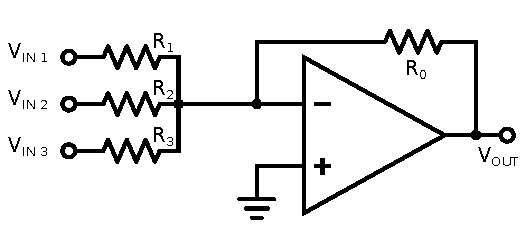
\includegraphics[width=65mm]{ccsum.pdf}
	\label{fig:ccsum}
\end{wrapfigure}

Il circuito riportato in Fig.(\ref{fig:ccsum}) è lo schema del circuito sommatore.
Tale circuito permette di sommare più segnali in input e risulta particolarmente comodo nel caso, ad esempio, della necessità di trasformare un segnale digitale (espresso in bit) in un segnale analogico (ampiezza).
Analizziamo il circuito sempre assumendo un op-amp ideale.
Anche in questo caso $V_A$ sarà un ground virtuale ($V_A = 0$).
Possiamo dunque imporre la seguente condizione: $\frac{V_1}{R_1}+\frac{V_2}{R_2}+\frac{V_3}{R_3}=\frac{-V_{out}}{R_0}$.
Dunque, se $R_0=R_1=R_2=R_3$ segue immediatamente che $V_{out}=V_1+V_2+V_3$.
Ne abbiamo verificato il funzionamento utilizzando diversi segnali in input (tra cui onde quadre, segnali DC, ecc.).

Nei seguenti grafici in Fig. \ref{fig:sum} sono riportati i segnali visualizzati a schermo sull'oscilloscopio per alcune combinazioni si segnali in input.

\begin{figure}[h]
	\centering
			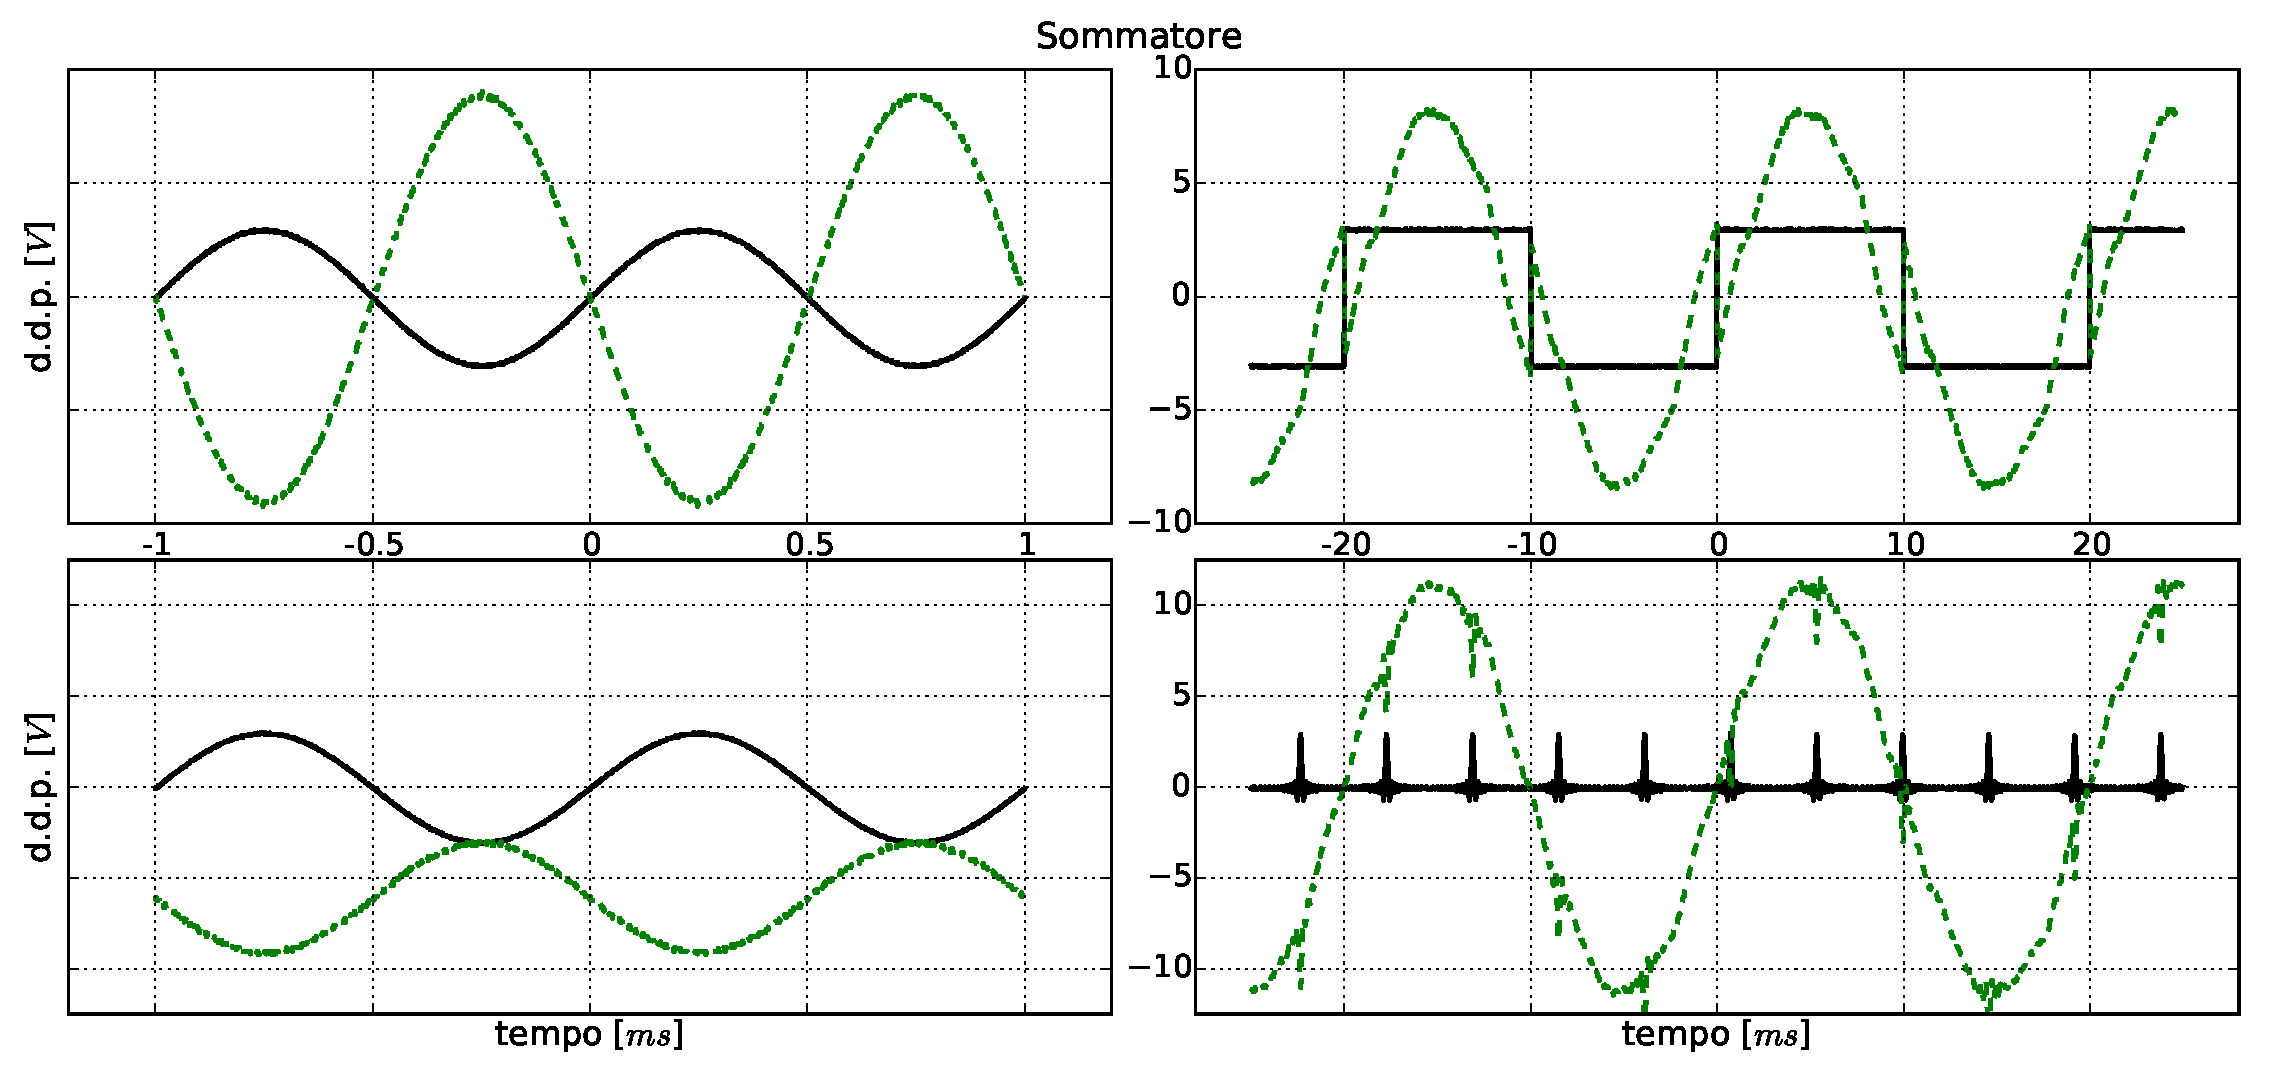
\includegraphics[width=.9\textwidth]{sum_serie_05.pdf}
			\caption{In nero possiamo vedere uno dei segnali in input mentre in verde tratteggiato il segnale in output. Nel primo grafico in alto a sinistra vediamo la somma di tre segnali sinusoidali identici. In quello a destra è stato aggiunto un segnale DC di +6V che evidentemente, per la natura del sommatore, porterà ad un offset di -6V. Nel terzo grafico in basso a sinistra possiamo vedere un'onda sinusoidale con sommata un'onda quadra mentre nell'ultimo grafico abbiamo sommato un cardiode ad una sinusoidale.}
			\label{fig:sum}
\end{figure}

È evidente che il circuito si comporti da sommatore. I valori di resistenza utilizzate sono stati $R_0=(10.01\pm0.02)$ \si{\kilo\ohm}, $R_1=(9.95\pm0.01)$ \si{\kilo\ohm}, $R_2=(10.02\pm 0.01)$ \si{\kilo\ohm} e $R_3=(9.97\pm0.01)$ \si{\kilo\ohm}. \phantom{xxxxxxxxxxxxxxxxxxxxxxxxxxxxxxxxxxxxxxxx}